\documentclass[sigconf]{acmart}

\usepackage[brazilian]{babel}
\usepackage{booktabs}
\usepackage{graphicx}
\usepackage{tabularx}
\setlength{\emergencystretch}{2em}

\setcopyright{none}
\settopmatter{printacmref=false}
\acmConference{Reprodutibilidade}{Julho de 2026}{Brasil}
\acmBooktitle{Reprodutibilidade: Projeto de Pesquisa -- Etapa 3}
\acmYear{2026}
\acmDOI{}
\acmISBN{}

\begin{document}
\renewcommand{\keywordsname}{PALAVRAS-CHAVE}

\title{Efeito do Número de Memórias Recuperadas no A-Mem: uma Replicação Parcial com Desenho em Blocos no LoCoMo}

\author{Patrick de \^{A}ngelis Am\^{a}ncio Meneses Santos}
\affiliation{%
  \institution{Programa de Pós-Graduação em Ciência da Computação (PPGCC)}
  \institution{Universidade Federal de Campina Grande (UFCG)}
  \city{Campina Grande}
  \state{Paraíba}
  \country{Brasil}
}

\begin{abstract}
Este trabalho apresenta uma replicação parcial do método e dos artefatos do A-Mem. O experimento avalia o efeito de memórias recuperadas por consulta, \(k\in\{3,5,10\}\), no primeiro diálogo do LoCoMo.

O limite de custo impediu o benchmark completo. O estudo fica condicionado a um diálogo com 19 sessões, 419 turnos e 199 perguntas, repetido em cinco blocos com ordem balanceada de \(k\).

Em todos os blocos, \(k=10\) superou \(k=3\). O delta médio de F1 foi 0,0960, IC bootstrap de 95\% [0,0806; 0,1136], teste exato de sinais unilateral \(p=0,03125\) e \(d_z=4,61\).

Os contrastes 3--5 e 5--10 foram positivos, mas inconclusivos após Holm. As durações registradas somaram 5,09 horas, sem o tempo da construção R1. O custo total é estimado em US\$2,52.

Código, dados, resultados, ambiente e hashes compõem o Kit de Reprodução. As conclusões não são generalizadas para o LoCoMo completo.
\end{abstract}

\keywords{memória de agentes, LLM, A-Mem, LoCoMo, experimentação, reprodutibilidade}

\maketitle

\section{Introdução}

Agentes baseados em grandes modelos de linguagem recuperam experiências anteriores para manter coerência. O A-Mem organiza essas experiências como notas interconectadas, inspirado no método Zettelkasten~\cite{xu2025amem}.

O LoCoMo é um dos benchmarks usados pelo A-Mem. Ele contém conversas extensas anotadas para resposta a perguntas e outras tarefas de memória~\cite{maharana2024locomo}.

O estudo original avalia dez diálogos, 1.986 perguntas, múltiplos modelos e baselines. Esse custo não era viável aqui.

Pela taxonomia adotada na disciplina, este trabalho é uma replicação parcial com extensão. Ele reutiliza código, dados e fluxo de avaliação, mas formula uma nova análise de sensibilidade de \texttt{retrieve\_k}.

Adotou-se um estudo de caso: fixar o \texttt{sample 0}, reconstruir a memória cinco vezes e comparar três níveis de recuperação. Perguntas correlacionadas não são tratadas como réplicas independentes.

A questão principal é se recuperar dez memórias aumenta o F1 médio em relação a recuperar três. Contrastes 3--5 e 5--10, métricas secundárias, tokens, duração e custo são análises adicionais.

As contribuições são um desenho em blocos, instrumentação de uso e custo, análise estatística regenerável e um Kit de Reprodução que refaz a análise sem custo de API.

\section{Metodologia}

\subsection{Sistema, dados e escopo}

O código-base é a implementação oficial do A-Mem, commit \texttt{0c8039f28fdc}~\cite{xu2025repo}. Esse hash identifica o código upstream, não as modificações locais exatas usadas na coleta.

O backend foi a OpenAI API com \texttt{gpt-4o-mini}. O dataset tem SHA-256 iniciado por \texttt{79fa87e90f04}. O \texttt{sample 0} contém 19 sessões, 419 turnos e 199 perguntas.

O recorte é determinístico, não uma amostra aleatória dos dez diálogos. As categorias 1 a 5 seguem o mapeamento oficial: multi-hop, temporal, open-domain, single-hop e adversarial.

As análises por categoria são exploratórias. Há apenas um diálogo, e algumas categorias contêm poucos casos.

\subsection{Desenho experimental}

A variável independente é \texttt{retrieve\_k}, com níveis 3, 5 e 10. Foram executadas cinco repetições separadas, R1 a R5. Cada repetição reconstruiu 419 memórias em cache próprio.

Dentro da repetição, os níveis compartilharam o cache. A agenda foi gerada antes da coleta com \texttt{schedule\_seed} igual a 20260714 e depois incluída no manifesto.

A agenda ainda não estava em um commit Git antes da coleta. Os metadados dos 15 resultados confirmam a ordem executada. Cada nível apareceu uma ou duas vezes em cada posição.

O bloco, não a pergunta, é a unidade de repetição. As 199 perguntas são casos fixos e correlacionados dentro de um diálogo.

Seeds lógicas foram \texttt{20260715} a \texttt{20260719}. Elas controlaram a agenda e geradores locais, mas não foram enviadas à OpenAI API. A temperatura foi 0,0 nas categorias 1--4 e 0,5 na adversarial.

\subsection{Hipóteses e métricas}

Para cada bloco \(r\), definiu-se \(d_r=F1_{r,k=10}-F1_{r,k=3}\). A hipótese nula é \(P(d_r>0)\leq0,5\); a alternativa é \(P(d_r>0)>0,5\), com \(\alpha=0,05\).

F1 médio foi o desfecho primário. Exact match, BLEU, ROUGE, METEOR e similaridades BERT/SBERT foram métricas secundárias. Categorias foram exploratórias.

Tokens, requisições, tentativas, falhas, duração e custo foram registrados por fase. Os preços por milhão de tokens foram US\$0,15 para entrada, US\$0,075 para cache e US\$0,60 para saída, em 14 de julho de 2026.

\subsection{Plano de análise}

O contraste primário usou teste exato de sinais unilateral. Com cinco deltas não nulos, a menor probabilidade unilateral é 0,03125. Os contrastes secundários usaram testes bilaterais e correção de Holm.

Reportam-se descritivas, diferença relativa, IC bootstrap de 95\% com 10.000 reamostragens e \(d_z\). Shapiro-Wilk é apenas diagnóstico; a decisão principal não depende de normalidade.

\section{Resultados}

\subsection{F1 por cenário e bloco}

As médias de F1 foram 0,2676 (DP 0,0108) para \(k=3\), 0,2943 (DP 0,0165) para \(k=5\) e 0,3636 (DP 0,0177) para \(k=10\). A Tabela~\ref{tab:f1-resumo} resume os cenários.

\begin{table}[htbp]
\centering
\caption{F1 médio entre os cinco blocos.}
\label{tab:f1-resumo}
\begin{tabular}{@{}rrrr@{}}
\toprule
\(k\) & Média & DP & Blocos \\
\midrule
3  & 0,2676 & 0,0108 & 5 \\
5  & 0,2943 & 0,0165 & 5 \\
10 & 0,3636 & 0,0177 & 5 \\
\bottomrule
\end{tabular}
\end{table}

\begin{figure}[htbp]
\centering
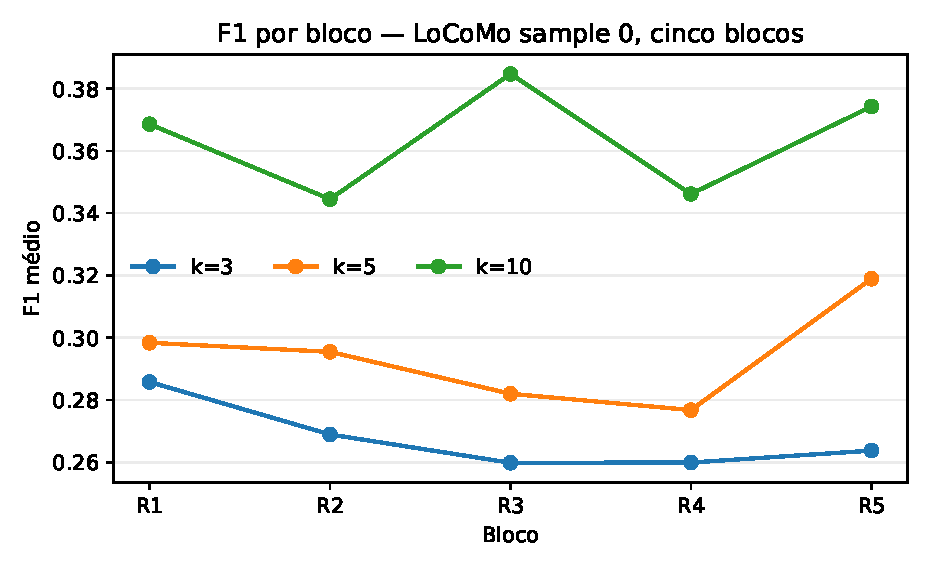
\includegraphics[width=\columnwidth]{assets/figures/f1_por_bloco.pdf}
\caption{F1 médio por bloco e valor de \(k\) no \texttt{sample 0}.}
\label{fig:f1-bloco}
\end{figure}

\subsection{Contrastes pareados}

Todos os cinco deltas 3--10 foram positivos. O ganho médio foi 0,0960, ou 35,9\% da média-base. O IC bootstrap de 95\% foi [0,0806; 0,1136].

O teste exato de sinais unilateral produziu \(p=0,03125\). Rejeita-se a hipótese nula no escopo condicionado às cinco repetições. O efeito foi \(d_z=4,61\), estimativa instável com \(n=5\).

Os deltas médios foram 0,0267 para 3--5 e 0,0693 para 5--10. Os testes bilaterais deram \(p=0,0625\) e \(p_{Holm}=0,125\). São evidências descritivas, não confirmações a 5\%.

\begin{table*}[htbp]
\centering
\caption{Contrastes pareados de F1 entre os cinco blocos.}
\label{tab:contrastes}
\begin{tabular}{@{}lrrrrrr@{}}
\toprule
Contraste & Delta médio & IC 95\% & Dif. relativa & \(p\) & \(p_{Holm}\) & \(d_z\) \\
\midrule
3--5  & 0,0267 & [0,0162; 0,0409] & 9,96\%  & 0,0625 & 0,1250 & 1,59 \\
3--10 & 0,0960 & [0,0806; 0,1136] & 35,87\% & 0,03125 unilateral & -- & 4,61 \\
5--10 & 0,0693 & [0,0556; 0,0867] & 23,56\% & 0,0625 & 0,1250 & 3,34 \\
\bottomrule
\end{tabular}
\end{table*}

Shapiro-Wilk produziu \(p=0,146\), \(p=0,406\) e \(p=0,381\) para 3--5, 3--10 e 5--10. O diagnóstico tem baixo poder com \(n=5\) e não escolheu o teste principal.

\begin{figure}[htbp]
\centering
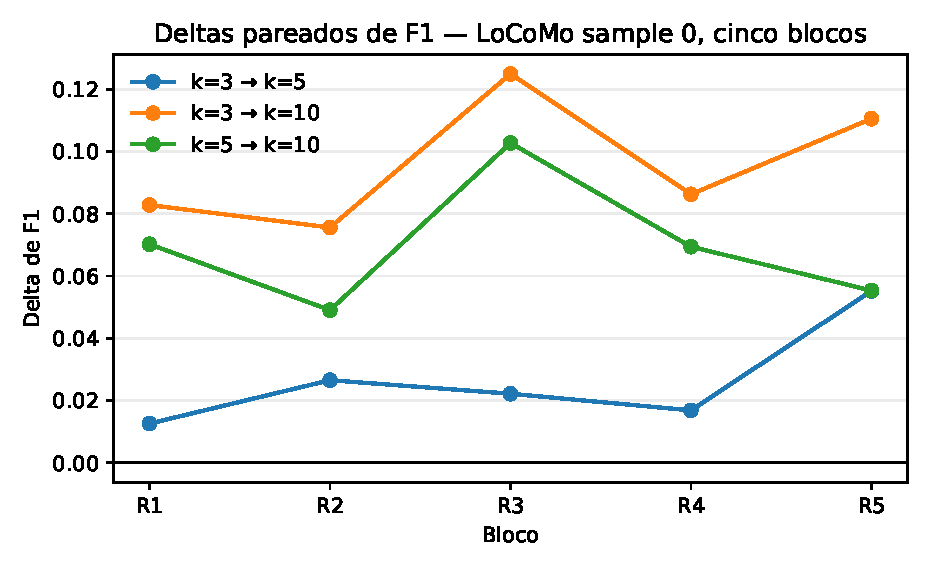
\includegraphics[width=\columnwidth]{assets/figures/deltas_f1.pdf}
\caption{Deltas pareados de F1 por bloco.}
\label{fig:deltas}
\end{figure}

\subsection{Métricas secundárias e categorias}

% Generated deterministically from the Entrega 3 analysis JSON.
\begin{table*}[t]
\centering
\caption{Médias entre blocos das métricas por cenário no LoCoMo sample 0.}
\label{tab:metricas-secundarias}
\begin{tabular}{rrrrrrr}
\toprule
$k$ & Exact match & F1 & ROUGE-1 F & METEOR & BERT F1 & SBERT \\
\midrule
3 & 0.093467 & 0.267630 & 0.279333 & 0.199038 & 0.894286 & 0.438117 \\
5 & 0.110553 & 0.294297 & 0.305085 & 0.221730 & 0.897298 & 0.460274 \\
10 & 0.145729 & 0.363631 & 0.374413 & 0.273141 & 0.907042 & 0.527424 \\
\bottomrule
\end{tabular}
\end{table*}


Todas as métricas agregadas cresceram de \(k=3\) para \(k=10\). Por exemplo, exact match passou de 0,0935 para 0,1457; METEOR, de 0,1990 para 0,2731; e SBERT, de 0,4381 para 0,5274.

BLEU-1 foi coletado e preservado nos JSONs, embora não apareça na tabela compacta. Sua média entre blocos cresceu de 0,2346 em \(k=3\) para 0,2571 em \(k=5\) e 0,3184 em \(k=10\).

O F1 por categoria aumentou de \(k=3\) para \(k=10\) em multi-hop, temporal, single-hop e adversarial. Em open-domain, \(k=5\) obteve 0,1299 e \(k=10\), 0,1281. Esses resultados são exploratórios.

\subsection{Custo, uso e tempo}

As durações gravadas somaram 5,09 horas, mas não incluem a construção R1. Houve 11.067 requisições concluídas e nenhuma tentativa falha. O custo registrado foi US\$2,3567.

O total inclui quatro construções de memória, por US\$0,6515, e todas as avaliações. A construção R1 terminou antes de salvar telemetria. Pela média das outras quatro, o custo global estimado é US\$2,52.

Na avaliação, tokens médios foram 370.800, 652.939 e 1.278.731 para \(k=3,5,10\). Os respectivos custos foram US\$0,0549, US\$0,0970 e US\$0,1892.

Os DP de tokens foram 3.874, 14.769 e 34.551; os DP de custo, US\$0,0023, US\$0,0023 e US\$0,0060. Mais memórias elevaram uso e custo.

A duração total por execução inclui a construção na primeira posição do bloco. Portanto, diferenças de duração por \(k\) estão confundidas pela ordem e não recebem interpretação causal.

\subsection{Comparação com o trabalho original}

O estudo original compara A-Mem com baselines no LoCoMo completo e em vários modelos. Esta replicação preserva arquitetura, benchmark e fluxo de avaliação, mas não repete essa comparação ampla.

Aqui, a pergunta é uma análise de sensibilidade de \texttt{retrieve\_k} em um diálogo e um modelo. O ganho com \(k=10\) mostra que a configuração de recuperação afeta o resultado local.

Esse achado não confirma a superioridade geral do A-Mem sobre baselines. Ele complementa o artigo original com evidência condicionada e identifica custo maior quando mais memórias são recuperadas.

\section{Ameaças à Validade}

A ameaça externa dominante é o único diálogo. Os resultados não estimam desempenho médio no LoCoMo e não devem ser extrapolados para outros diálogos, modelos ou versões de API.

As 199 perguntas compartilham memória e contexto. Tratá-las como 199 réplicas independentes produziria inferência otimista.

Cinco blocos oferecem resolução limitada. O resultado atinge o menor \(p\) unilateral possível porque os cinco sinais são positivos. Isso sustenta a direção local, mas não substitui mais diálogos.

IC bootstrap e \(d_z\) são instáveis com cinco blocos. Devem ser interpretados junto aos deltas individuais.

As seeds não foram enviadas à API. Mesmo com temperatura controlada, respostas hospedadas não são bit a bit determinísticas. Mudanças de modelo ou infraestrutura podem afetar reproduções futuras.

Métricas automáticas podem penalizar respostas semanticamente equivalentes. Resultados por categoria têm poucos casos e são exploratórios.

Em R1, \texttt{punkt\_tab} não estava no preflight. A falha ocorreu após salvar o cache e na primeira pergunta. A avaliação foi retomada sem reconstruir a memória.

O cache e os resultados foram preservados, mas tempo e uso da construção R1 ficaram ausentes. Nenhuma execução foi repetida ou excluída por desempenho.

O commit nos JSONs identifica o upstream. As mudanças locais usadas na coleta ainda não estavam commitadas, e a agenda não possuía comprovação Git anterior. Essa limitação retrospectiva não pode ser eliminada.

\section{Reprodutibilidade e Kit de Reprodução}

O Kit de Reprodução está no
\href{https://github.com/patrickdeangelis/amem-locomo-replication}{repositório público no GitHub},
no commit \texttt{5b28c7a5c1b9}. Depósito arquivístico e DOI permanecem pendentes.

O código-base usa MIT; o LoCoMo, CC BY-NC 4.0. Artigo, documentação e derivados locais usam CC BY 4.0, conforme \path{LICENSE-ARTIFACTS.md}.

O kit contém o código usado, ambiente travado, dataset, agenda, 15 JSONs, análise, testes, tabelas, figuras, protocolo e o artigo final em PDF e em fonte \LaTeX. A publicação do fonte permite inspecionar e recompilar o manuscrito, enquanto os resultados e ativos derivados permanecem rastreáveis pelo manifesto de hashes.

O ambiente foi macOS 26.4 arm64 em MacBook Pro com Apple M1 Pro, 10 núcleos, 16 GB de RAM e Python 3.11.15. Detalhes estão em \path{experiments/retrieve-k-five-blocks/environment.md}.

Após clonar o repositório indicado, os comandos abaixo instalam o ambiente, executam os testes públicos e regeneram análise e derivados:

\begin{verbatim}
cd amem
python3.11 -m venv .venv
. .venv/bin/activate
pip install -r requirements.lock.txt
python -m pytest tests -q
\end{verbatim}

O README fornece os comandos completos para executar \texttt{analyze\_entrega3.py} sobre os 15 JSONs e exportar tabelas e figuras. Esses passos não exigem chave nem custo de API.

Para refazer chamadas, configura-se \texttt{.env.local}. A execução paga exige o comando \texttt{python run\_entrega3.py --execute}.

O runner não chama a API sem \texttt{--execute}. A agenda existente não é reescrita se divergir do plano. Somente JSONs completos, com 199 perguntas e metadados consistentes, são aceitos como válidos.

A coleta registrou 5,09 horas, acrescidas do tempo não registrado da construção R1. O custo total estimado é US\$2,52. Respostas futuras podem se aproximar, mas não coincidir bit a bit.

\section{Conclusões}

No \texttt{sample 0}, aumentar \(k\) de 3 para 10 elevou o F1 nas cinco repetições. O ganho médio foi 0,0960, com \(p=0,03125\). Contrastes intermediários foram inconclusivos após Holm.

Métricas secundárias acompanharam a direção do F1. Recuperar mais memórias também elevou tokens e custo de avaliação.

O resultado sustenta a hipótese condicionada ao diálogo, não uma afirmação sobre o LoCoMo completo nem sobre superioridade frente aos baselines originais.

A continuidade científica é repetir o desenho em mais diálogos. Dentro do limite financeiro, o projeto produz uma comparação sustentada, auditável e reproduzível.

\bibliographystyle{ACM-Reference-Format}
\begin{thebibliography}{3}

\bibitem{maharana2024locomo}
Adyasha Maharana, Dong-Ho Lee, Sergey Tulyakov, Mohit Bansal, Francesco Barbieri, and Yuwei Fang. 2024.
Evaluating Very Long-Term Conversational Memory of LLM Agents.
In \textit{Proceedings of ACL 2024}, 13851--13870.
\url{https://doi.org/10.18653/v1/2024.acl-long.747}

\bibitem{xu2025repo}
Wujiang Xu. 2025.
A-Mem: Agentic Memory for LLM Agents -- código oficial.
\url{https://github.com/WujiangXu/A-mem}

\bibitem{xu2025amem}
Wujiang Xu, Zujie Liang, Kai Mei, Hang Gao, Juntao Tan, and Yongfeng Zhang. 2025.
A-Mem: Agentic Memory for LLM Agents.
In \textit{Advances in Neural Information Processing Systems}.
\url{https://doi.org/10.48550/arXiv.2502.12110}

\end{thebibliography}
\end{document}
